% Figure 1 v8 — Wang KBS layout: 3 stacked rows (full-width per row).
% Row 1: Stage A · Inputs (3 horizontal panels)
% Row 2: Stage B · Encoder (3 horizontal panels: static / dynamic / fusion)
% Row 3: Stage C · Choice head + Loss + Trained Θ output card
%
% Compile:  pdflatex figure1_architecture_v8.tex

\documentclass[border=8pt]{standalone}

\usepackage[T1]{fontenc}
\usepackage{lmodern}
\usepackage{amsmath, amssymb}
\usepackage{tikz}
\usepackage{xcolor}
\usepackage{graphicx}

\usetikzlibrary{
  positioning, arrows.meta, shapes.geometric, calc, fit, backgrounds,
  matrix, decorations.pathmorphing,
}

\definecolor{stageABg}    {HTML}{E0EBF5}
\definecolor{stageABanner}{HTML}{3B6FB6}
\definecolor{stageBBg}    {HTML}{E6F1E5}
\definecolor{stageBBanner}{HTML}{2E7D32}
\definecolor{stageCBg}    {HTML}{FAE5DD}
\definecolor{stageCBanner}{HTML}{C44E52}
\definecolor{cFlow}       {HTML}{E07A5F}
\definecolor{cBack}       {HTML}{8B5CF6}
\definecolor{cText}       {HTML}{1F2937}
\definecolor{cMuted}      {HTML}{6B7280}
\definecolor{cBorder}     {HTML}{CBD5E1}
\definecolor{cIO}         {HTML}{0F766E}

% Tensor cell category colours
\definecolor{cPOI}      {HTML}{93C5FD}
\definecolor{cSector}   {HTML}{86EFAC}
\definecolor{cEmp}      {HTML}{FDBA74}
\definecolor{cPop}      {HTML}{FDE68A}
\definecolor{cIMD}      {HTML}{FCA5A5}
\definecolor{cTube}     {HTML}{C4B5FD}

% Mixture utility 4-term colours
\definecolor{cTermV}    {HTML}{8172B2}
\definecolor{cTermBeta} {HTML}{C44E52}
\definecolor{cTermGamma}{HTML}{F59E0B}
\definecolor{cTermDelta}{HTML}{0E7490}

% Parameter category colours
\definecolor{cParEnc}   {HTML}{475569}
\definecolor{cParBeta}  {HTML}{C44E52}
\definecolor{cParGamma} {HTML}{F59E0B}
\definecolor{cParDelta} {HTML}{0E7490}
\definecolor{cParKappa} {HTML}{8172B2}

% Agent type colours (consistent with agent_heterogeneity icon)
\definecolor{cAgentWalk}   {HTML}{10B981}
\definecolor{cAgentTransit}{HTML}{F59E0B}
\definecolor{cAgentCar}    {HTML}{3B82F6}

\newcommand{\rowwidth}{300mm}    % uniform row width

\begin{document}

\begin{tikzpicture}[
  font=\sffamily\small,
  thick,
  >={Stealth[length=4.5pt, width=4pt]},
  every node/.style={align=center, text=cText},
  %
  rowframe/.style={
    draw=none, fill=#1, rounded corners=6pt,
    inner xsep=8pt, inner ysep=10pt,
  },
  rowbanner/.style={
    fill=#1, text=white, font=\sffamily\bfseries\small,
    rounded corners=4pt, inner sep=6pt,
  },
  modA/.style={
    draw=stageABanner, fill=white, line width=0.7pt,
    rounded corners=3pt, inner sep=5pt,
  },
  modB/.style={
    draw=stageBBanner, fill=white, line width=0.7pt,
    rounded corners=3pt, inner sep=5pt,
  },
  modC/.style={
    draw=stageCBanner, fill=white, line width=0.7pt,
    rounded corners=3pt, inner sep=5pt,
  },
  arrFwd/.style={->, line width=1.6pt, draw=cFlow},
  arrInner/.style={->, line width=0.8pt, draw=cText!70},
  arrBack/.style={->, line width=1.0pt, draw=cBack, dashed},
  arrlbl/.style={font=\sffamily\scriptsize\itshape, text=cMuted, fill=white,
                 inner sep=1pt, midway},
  cellgrid/.style={draw=cMuted!50, fill=#1, line width=0.3pt, rectangle},
]

% ════════════════════════════════════════════════════════════════════════
%  ROW 1 · STAGE A · INPUTS  (7 horizontal panels with encoder/choice divider)
%  Left group  (3 panels): X^static, X^dyn, G — go through ENCODER
%  Right group (4 panels): t^(m), log d, OccMatch, π_m+π_k — skip encoder,
%                          go DIRECTLY to choice head
% ════════════════════════════════════════════════════════════════════════

\begin{scope}[local bounding box=row1]

  % ────────── LEFT GROUP: ENCODER INPUTS ──────────

  % Panel 1: X^static
  \node[modA, anchor=north west] (xstatic) at (0, 0)
    {\begin{minipage}{52mm}
      \centering\textbf{\textcolor{stageABanner}{$X^{\text{static}}$}}\;\scriptsize $\mathbb{R}^{N\!\times\!22}$\\\tiny\textcolor{cMuted}{node features}\\[3pt]
      \begin{tikzpicture}[scale=0.78, baseline=0]
        \node[font=\sffamily\tiny] at (1.5*2.5mm, 2mm) {POI};
        \node[font=\sffamily\tiny] at (7.5*2.5mm, 2mm) {sectors};
        \node[font=\sffamily\tiny] at (12.5*2.5mm, 2mm) {emp};
        \node[font=\sffamily\tiny] at (14.5*2.5mm, 2mm) {pop};
        \node[font=\sffamily\tiny] at (16*2.5mm, 2mm) {IMD};
        \node[font=\sffamily\tiny] at (19*2.5mm, 2mm) {tube};
        \foreach \r in {0,...,4} {
          \foreach \c in {0,1,2,3}
            \node[cellgrid=cPOI, minimum size=2.5mm] at (\c*2.5mm, -\r*2.5mm) {};
          \foreach \c [evaluate=\c as \cc using int(\c+4)] in {0,...,7}
            \node[cellgrid=cSector, minimum size=2.5mm] at (\cc*2.5mm, -\r*2.5mm) {};
          \foreach \c [evaluate=\c as \cc using int(\c+12)] in {0,1}
            \node[cellgrid=cEmp, minimum size=2.5mm] at (\cc*2.5mm, -\r*2.5mm) {};
          \foreach \c [evaluate=\c as \cc using int(\c+14)] in {0,1}
            \node[cellgrid=cPop, minimum size=2.5mm] at (\cc*2.5mm, -\r*2.5mm) {};
          \node[cellgrid=cIMD, minimum size=2.5mm] at (16*2.5mm, -\r*2.5mm) {};
          \foreach \c [evaluate=\c as \cc using int(\c+17)] in {0,...,4}
            \node[cellgrid=cTube, minimum size=2.5mm] at (\cc*2.5mm, -\r*2.5mm) {};
        }
        \node[font=\sffamily\tiny, text=cMuted] at (10*2.5mm, -6.5*2.5mm) {$\vdots\;1725$ rows · time-invariant};
      \end{tikzpicture}
    \end{minipage}};

  % Panel 2: X^dyn
  \node[modA, anchor=north west] (xdyn) at (62mm, 0)
    {\begin{minipage}{52mm}
      \centering\textbf{\textcolor{stageABanner}{$X^{\text{dyn}}$}}\;\scriptsize $\mathbb{R}^{T\!\times\!N\!\times\!5}$\\\tiny\textcolor{cMuted}{hourly features}\\[3pt]
      \begin{tikzpicture}[baseline=0]
        \begin{scope}[shift={(0,0)}]
          \foreach \r in {0,...,3} {
            \foreach \c in {0,...,4} {
              \node[cellgrid=stageABanner, minimum size=2.0mm,
                     opacity={0.30+0.15*\r}]
                    at (\c*2.0mm, -\r*2.0mm) {};
            }
          }
          \draw[fill=stageABanner!30, opacity=0.6, line width=0.3pt]
            (0, 0.8mm) -- (5*2.0mm, 0.8mm) -- (5*2.0mm + 6mm, 4mm) -- (6mm, 4mm) -- cycle;
          \draw[fill=stageABanner!20, opacity=0.6, line width=0.3pt]
            (5*2.0mm, 0.8mm) -- (5*2.0mm + 6mm, 4mm)
              -- (5*2.0mm + 6mm, 4mm - 4*2.0mm) -- (5*2.0mm, -3*2.0mm) -- cycle;
          \node[font=\sffamily\tiny, text=cMuted] at (-3mm, -3mm) {$N$};
          \node[font=\sffamily\tiny, text=cMuted] at (5mm, 5mm) {$T{=}24$};
          \node[font=\sffamily\tiny, text=cMuted] at (5*2.0mm + 8mm, -2mm) {$F{=}5$};
        \end{scope}
        \node[font=\sffamily\tiny, text=cText, anchor=west]
          at (24mm, 2mm) {cong z · inflow z};
        \node[font=\sffamily\tiny, text=cText, anchor=west]
          at (24mm, -1mm) {queue · sin/cos $h$};
        \node[font=\sffamily\tiny, text=cMuted] at (16mm, -14mm) {1725 grids $\times$ 24 h};
      \end{tikzpicture}
    \end{minipage}};

  % Panel 3: G (graph)
  \node[modA, anchor=north west] (xgraph) at (124mm, 0)
    {\begin{minipage}{40mm}
      \centering\textbf{\textcolor{stageABanner}{$\mathcal{G}\!=\!(V,E)$}}\;\\\tiny\textcolor{cMuted}{edge\_index, derived}\\[3pt]
      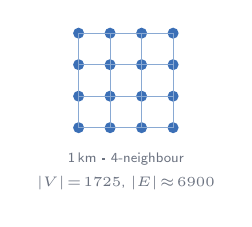
\begin{tikzpicture}[baseline=0]
        \foreach \x/\y/\name in
          {0/0/n00, 1/0/n10, 2/0/n20, 3/0/n30,
           0/1/n01, 1/1/n11, 2/1/n21, 3/1/n31,
           0/2/n02, 1/2/n12, 2/2/n22, 3/2/n32,
           0/3/n03, 1/3/n13, 2/3/n23, 3/3/n33}{
          \node[circle, fill=stageABanner, minimum size=1.4mm, inner sep=0pt]
                (\name) at (\x*4mm, -\y*4mm) {};
        }
        \foreach \y in {0,1,2,3}{
          \foreach \x in {0,1,2}{
            \pgfmathtruncatemacro{\xn}{\x+1}
            \draw[stageABanner!60, line width=0.3pt] (\x*4mm, -\y*4mm) -- (\xn*4mm, -\y*4mm);
          }
        }
        \foreach \x in {0,1,2,3}{
          \foreach \y in {0,1,2}{
            \pgfmathtruncatemacro{\yn}{\y+1}
            \draw[stageABanner!60, line width=0.3pt] (\x*4mm, -\y*4mm) -- (\x*4mm, -\yn*4mm);
          }
        }
        \node[font=\sffamily\tiny, text=cMuted] at (6mm, -16mm) {1\,km · 4-neighbour};
        \node[font=\sffamily\tiny, text=cMuted] at (6mm, -19mm) {$|V|\!=\!1725$, $|E|\!\approx\!6900$};
      \end{tikzpicture}
    \end{minipage}};

  % ────────── DIVIDER ──────────
  \draw[dashed, line width=0.6pt, draw=cMuted]
        (172mm, 8mm) -- (172mm, -34mm);
  \node[font=\sffamily\scriptsize\itshape, text=stageABanner, anchor=south]
        at (87mm, 8mm) {$\downarrow$ to ENCODER (Stage B)};
  \node[font=\sffamily\scriptsize\itshape, text=stageBBanner, anchor=south]
        at (240mm, 8mm) {$\downarrow$ direct to CHOICE HEAD (skip encoder)};

  % ────────── RIGHT GROUP: CHOICE HEAD INPUTS ──────────

  % Panel 4: t_{ij}^{(m)} — 3 stacked mode heatmaps
  \node[modA, anchor=north west, draw=stageBBanner] (tij) at (180mm, 0)
    {\begin{minipage}{32mm}
      \centering\textbf{\textcolor{stageBBanner}{$t_{ij}^{(m)}$}}\;\scriptsize $\mathbb{R}^{N\!\times\!N\!\times\!3}$\\\tiny\textcolor{cMuted}{travel time per mode}\\[3pt]
      \begin{tikzpicture}[baseline=0]
        \foreach \mname/\yoff/\col in {car/0/cAgentCar, transit/-7mm/cAgentTransit, walk/-14mm/cAgentWalk}{
          \node[font=\sffamily\tiny, text=\col, anchor=east] at (-1mm, \yoff) {\mname};
          \foreach \c in {0,...,9}{
            \pgfmathsetmacro{\val}{0.2 + 0.07*\c}
            \node[cellgrid=cTermBeta, minimum size=1.5mm, opacity=\val]
                  at (\c*1.5mm, \yoff) {};
          }
        }
        \node[font=\sffamily\tiny, text=cMuted] at (8mm, -19mm) {$\to \beta_{t,m}\!\cdot\! t$};
      \end{tikzpicture}
    \end{minipage}};

  % Panel 5: log d_{ij} — distance decay
  \node[modA, anchor=north west, draw=stageBBanner] (logd) at (216mm, 0)
    {\begin{minipage}{28mm}
      \centering\textbf{\textcolor{stageBBanner}{$\log d_{ij}$}}\;\scriptsize $\mathbb{R}^{N\!\times\!N}$\\\tiny\textcolor{cMuted}{Euclidean log-distance}\\[3pt]
      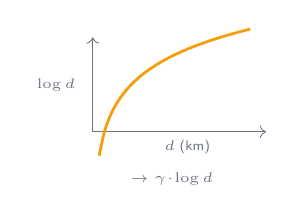
\begin{tikzpicture}[baseline=0]
        \draw[->, line width=0.3pt, draw=cMuted] (0, 0) -- (22mm, 0);
        \draw[->, line width=0.3pt, draw=cMuted] (0, 0) -- (0, 12mm);
        \draw[cTermGamma, line width=1.0pt, smooth, samples=30, domain=0.2:5]
              plot (\x*4mm, {ln(\x)*5mm + 5mm});
        \node[font=\sffamily\tiny, text=cMuted] at (12mm, -2mm) {$d$ (km)};
        \node[font=\sffamily\tiny, text=cMuted, anchor=east] at (-1mm, 6mm) {$\log d$};
        \node[font=\sffamily\tiny, text=cMuted] at (10mm, -6mm) {$\to \gamma\!\cdot\!\log d$};
      \end{tikzpicture}
    \end{minipage}};

  % Panel 6: OccMatch_{ij}
  \node[modA, anchor=north west, draw=stageBBanner] (occm) at (248mm, 0)
    {\begin{minipage}{30mm}
      \centering\textbf{\textcolor{stageBBanner}{OccMatch$_{ij}$}}\;\scriptsize $\mathbb{R}^{N\!\times\!N}$\\\tiny\textcolor{cMuted}{cosine-sim, SOC9$\!\times$sector}\\[3pt]
      \begin{tikzpicture}[baseline=0]
        \foreach \r in {0,...,7}{
          \foreach \c in {0,...,7}{
            \pgfmathsetmacro{\val}{0.1 + 0.5*rnd}
            \node[cellgrid=cTermDelta, minimum size=1.5mm, opacity=\val]
                  at (\c*1.5mm, -\r*1.5mm) {};
          }
        }
        \node[font=\sffamily\tiny, text=cMuted] at (6mm, -14mm) {origin job $\times$ dest sector};
        \node[font=\sffamily\tiny, text=cMuted] at (6mm, -17mm) {$\to \delta_k\!\cdot\!$OccM};
      \end{tikzpicture}
    \end{minipage}};

  % Panel 7: π_m + π_k — heterogeneity priors
  \node[modA, anchor=north west, draw=stageBBanner] (pies) at (282mm, 0)
    {\begin{minipage}{40mm}
      \centering\textbf{\textcolor{stageBBanner}{$\pi_m, \pi_k$}}\;\scriptsize priors\\\tiny\textcolor{cMuted}{mixture weights}\\[3pt]
      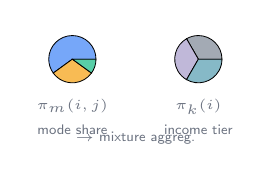
\begin{tikzpicture}[baseline=0]
        \begin{scope}[shift={(4mm, -4mm)}]
          \draw[fill=cAgentCar!70, line width=0.3pt] (0,0) -- (0:3mm) arc (0:216:3mm) -- cycle;
          \draw[fill=cAgentTransit!70, line width=0.3pt] (0,0) -- (216:3mm) arc (216:324:3mm) -- cycle;
          \draw[fill=cAgentWalk!70, line width=0.3pt] (0,0) -- (324:3mm) arc (324:360:3mm) -- cycle;
          \node[font=\sffamily\tiny, text=cMuted] at (0, -6mm) {$\pi_m(i,j)$};
          \node[font=\sffamily\tiny, text=cMuted] at (0, -9mm) {mode share};
        \end{scope}
        \begin{scope}[shift={(20mm, -4mm)}]
          \draw[fill=cParEnc!50, line width=0.3pt] (0,0) -- (0:3mm) arc (0:120:3mm) -- cycle;
          \draw[fill=cParKappa!50, line width=0.3pt] (0,0) -- (120:3mm) arc (120:240:3mm) -- cycle;
          \draw[fill=cParDelta!50, line width=0.3pt] (0,0) -- (240:3mm) arc (240:360:3mm) -- cycle;
          \node[font=\sffamily\tiny, text=cMuted] at (0, -6mm) {$\pi_k(i)$};
          \node[font=\sffamily\tiny, text=cMuted] at (0, -9mm) {income tier};
        \end{scope}
        \node[font=\sffamily\tiny, text=cMuted] at (12mm, -14mm) {$\to$ mixture aggreg.};
      \end{tikzpicture}
    \end{minipage}};

\end{scope}

\begin{pgfonlayer}{background}
  \node[rowframe=stageABg, fit=(row1)] (frameRow1) {};
\end{pgfonlayer}
\node[rowbanner=stageABanner, anchor=north west]
  at ($(frameRow1.north west)+(8pt, 0pt)$)
  {\textsc{Stage A · Inputs}\;\,\textmd{\itshape — encoder inputs (left) $+$ choice-head inputs (right, skip encoder)}};

% ════════════════════════════════════════════════════════════════════════
%  ROW 2 · STAGE B · ENCODER  (static / dynamic / fusion horizontal)
% ════════════════════════════════════════════════════════════════════════

\begin{scope}[local bounding box=row2, shift={(0, -80mm)}]

  % ── ① Static branch ──
  \node[modB, anchor=north west] (sage) at (0, 0)
    {\begin{minipage}{72mm}
      \centering\textbf{\textcolor{stageBBanner}{\textcircled{\scriptsize 1} Static branch · GraphSAGE $\times 2$}}\\[1pt]
      \scriptsize\textcolor{cIO}{IN: $X^{\text{static}}, \mathcal{G}$}\;\;\textcolor{cIO}{OUT: $h_s\!\in\!\mathbb{R}^{N\!\times\!32}$}\\[3pt]
      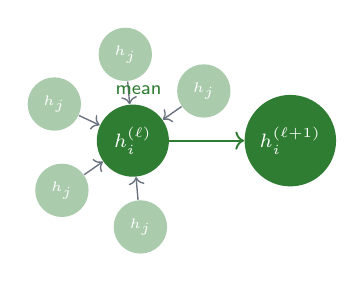
\begin{tikzpicture}[baseline=0]
        \node[circle, fill=stageBBanner, minimum size=6mm, font=\sffamily\scriptsize, text=white]
          (hi) at (0, 0) {$h_i^{(\ell)}$};
        \foreach \angle/\name in {35/n1, 95/n2, 155/n3, 215/n4, 275/n5}{
          \node[circle, fill=stageBBanner!40, minimum size=4mm,
                 font=\sffamily\tiny, text=white]
                (\name) at ({\angle}:11mm) {$h_j$};
          \draw[->, line width=0.5pt, draw=cMuted] (\name) -- (hi);
        }
        \node[font=\sffamily\scriptsize, text=stageBBanner, anchor=south]
           at (hi.north) {\;\;mean};
        \node[circle, fill=stageBBanner, minimum size=6mm, font=\sffamily\scriptsize, text=white]
          (hi1) at (20mm, 0) {$h_i^{(\ell{+}1)}$};
        \draw[->, line width=0.7pt, draw=stageBBanner] (hi.east) -- (hi1.west);
      \end{tikzpicture}\\[2pt]
      \scriptsize $h_i^{(\ell+1)}=\sigma\big(W^{(\ell)}\!\cdot\!\mathrm{mean}_{j\in\mathcal{N}(i)} h_j^{(\ell)}\big)$\\
      \tiny\textcolor{cMuted}{layer 1: $W^{(1)}{:}\,22{\to}32$;\;\;layer 2: $W^{(2)}{:}\,32{\to}32$}
    \end{minipage}};

  % ── ② Dynamic branch (absolute X) ──
  \node[modB, anchor=north west] (dyn) at (82mm, 0)
    {\begin{minipage}{146mm}
      \centering\textbf{\textcolor{stageBBanner}{\textcircled{\scriptsize 2} Dynamic branch · per-hour SAGE $\to$ GRU $\to$ multi-scale TCN $\to$ fuse}}\\[1pt]
      \scriptsize\textcolor{cIO}{IN: $X^{\text{dyn}}, \mathcal{G}$}\;\;\textcolor{cIO}{OUT: $h_d\!\in\!\mathbb{R}^{T\!\times\!N\!\times\!32}$}\\[3pt]
      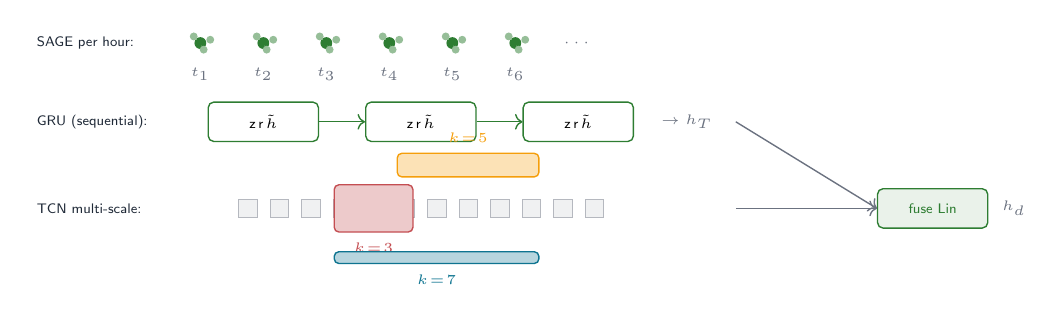
\begin{tikzpicture}[baseline=0]
        % per-hour SAGE
        \node[font=\sffamily\tiny, text=cText, anchor=west] at (0, 18mm) {SAGE per hour:};
        \foreach \t/\xoff in {1/22, 2/30, 3/38, 4/46, 5/54, 6/62}{
          \begin{scope}[shift={(\xoff mm, 18mm)}, scale=0.42]
            \node[circle, fill=stageBBanner, minimum size=1.5mm, inner sep=0pt] (a\t) at (0,0) {};
            \node[circle, fill=stageBBanner!50, minimum size=1.0mm, inner sep=0pt] (b\t) at (3mm, 1mm) {};
            \node[circle, fill=stageBBanner!50, minimum size=1.0mm, inner sep=0pt] (c\t) at (-2mm, 2mm) {};
            \node[circle, fill=stageBBanner!50, minimum size=1.0mm, inner sep=0pt] (d\t) at (1mm, -2mm) {};
            \draw[stageBBanner!50, line width=0.2pt] (a\t)--(b\t) (a\t)--(c\t) (a\t)--(d\t);
          \end{scope}
          \node[font=\sffamily\tiny, text=cMuted] at (\xoff mm, 14mm) {$t_\t$};
        }
        \node[font=\sffamily\tiny, text=cMuted] at (70mm, 18mm) {$\cdots$};
        % GRU row
        \node[font=\sffamily\tiny, text=cText, anchor=west] at (0, 8mm) {GRU (sequential):};
        \foreach \t/\xoff in {1/30, 2/50, 3/70}{
          \node[draw=stageBBanner, rounded corners=2pt, fill=white, line width=0.5pt,
                 minimum width=14mm, minimum height=5mm,
                 font=\sffamily\tiny] (gru\t) at (\xoff mm, 8mm) {z\,r\,$\tilde h$};
        }
        \draw[->, line width=0.5pt, draw=stageBBanner] (gru1.east) -- (gru2.west);
        \draw[->, line width=0.5pt, draw=stageBBanner] (gru2.east) -- (gru3.west);
        \node[font=\sffamily\tiny, text=cMuted] at (84mm, 8mm) {$\!\to h_T$};
        % TCN row
        \node[font=\sffamily\tiny, text=cText, anchor=west] at (0, -3mm) {TCN multi-scale:};
        \foreach \i in {0,...,11}{
          \node[draw=cMuted!50, fill=cMuted!10, minimum size=2mm, line width=0.2pt]
                at (28mm + \i*4mm, -3mm) {};
        }
        \draw[draw=cTermBeta, fill=cTermBeta!30, line width=0.5pt, rounded corners=0.6mm]
              (28mm + 3*4mm - 1mm, -6mm) rectangle (28mm + 5*4mm + 1mm, 0mm);
        \node[font=\sffamily\tiny, text=cTermBeta] at (28mm + 4*4mm, -8mm) {$k\!=\!3$};
        \draw[draw=cTermGamma, fill=cTermGamma!30, line width=0.5pt, rounded corners=0.6mm]
              (28mm + 5*4mm - 1mm, 1mm) rectangle (28mm + 9*4mm + 1mm, 4mm);
        \node[font=\sffamily\tiny, text=cTermGamma] at (28mm + 7*4mm, 6mm) {$k\!=\!5$};
        \draw[draw=cTermDelta, fill=cTermDelta!30, line width=0.5pt, rounded corners=0.6mm]
              (28mm + 3*4mm - 1mm, -10mm) rectangle (28mm + 9*4mm + 1mm, -8.5mm);
        \node[font=\sffamily\tiny, text=cTermDelta] at (28mm + 6*4mm, -12mm) {$k\!=\!7$};
        % fuse Lin
        \node[draw=stageBBanner, rounded corners=2pt, fill=stageBBanner!10,
               line width=0.5pt, minimum width=14mm, minimum height=5mm,
               font=\sffamily\tiny, text=stageBBanner]
              (fuse) at (115mm, -3mm) {fuse Lin};
        \draw[->, line width=0.5pt, draw=cMuted] (90mm, 8mm) -- (fuse.west);
        \draw[->, line width=0.5pt, draw=cMuted] (90mm, -3mm) -- (fuse.west);
        \node[font=\sffamily\tiny, text=cMuted, anchor=west] at (fuse.east) {\;$h_d$};
      \end{tikzpicture}
    \end{minipage}};

  % ── ③ Gated fusion (absolute X) ──
  \node[modB, anchor=north west] (gfuse) at (238mm, 0)
    {\begin{minipage}{60mm}
      \centering\textbf{\textcolor{stageBBanner}{\textcircled{\scriptsize 3} Gated fusion}}\\[1pt]
      \scriptsize\textcolor{cIO}{IN: $h_s, h_d$}\;\;\textcolor{cIO}{OUT: $V_{j,t}\!\in\!\mathbb{R}^{T\!\times\!N}$}\\[3pt]
      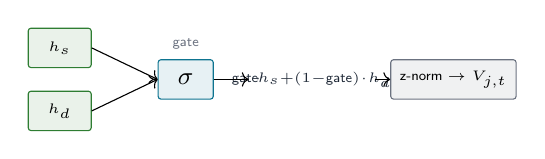
\begin{tikzpicture}[baseline=0]
        \node[draw=stageBBanner, fill=stageBBanner!10, rounded corners=1pt,
               minimum width=8mm, minimum height=5mm, font=\sffamily\tiny] (hs) at (0, 4mm) {$h_s$};
        \node[draw=stageBBanner, fill=stageBBanner!10, rounded corners=1pt,
               minimum width=8mm, minimum height=5mm, font=\sffamily\tiny] (hd) at (0, -4mm) {$h_d$};
        \node[draw=cTermDelta, fill=cTermDelta!10, rounded corners=1pt,
               minimum width=7mm, minimum height=5mm, font=\sffamily\small] (sig) at (16mm, 0) {$\sigma$};
        \draw[->, line width=0.4pt] (hs.east) -- (sig.west);
        \draw[->, line width=0.4pt] (hd.east) -- (sig.west);
        \node[font=\sffamily\tiny, text=cMuted, anchor=south] at (sig.north) {gate};
        \node[font=\sffamily\tiny, text=cText] at (32mm, 0) {gate$\!\cdot\!h_s$\\$+(1{-}$gate$)\!\cdot\!h_d$};
        \draw[->, line width=0.4pt] (sig.east) -- (24mm, 0);
        \node[draw=cMuted, fill=cMuted!10, rounded corners=1pt,
               minimum width=12mm, minimum height=5mm, font=\sffamily\tiny] (zn) at (50mm, 0) {z-norm $\to V_{j,t}$};
        \draw[->, line width=0.4pt] (40mm, 0) -- (zn.west);
      \end{tikzpicture}
    \end{minipage}};

  % inner arrows
  \draw[arrInner] (sage.east) -- node[arrlbl, above]{$h_s$} (dyn.west);
  \draw[arrInner] (dyn.east) -- node[arrlbl, above]{$h_d$} (gfuse.west);

\end{scope}

\begin{pgfonlayer}{background}
  \node[rowframe=stageBBg, fit=(row2)] (frameRow2) {};
\end{pgfonlayer}
\node[rowbanner=stageBBanner, anchor=north west]
  at ($(frameRow2.north west)+(8pt, 0pt)$)
  {\textsc{Stage B · Encoder}\;\,\textmd{\itshape — dual-branch ST-GNN $+$ gated fusion · 33{,}026 weights}};

% ════════════════════════════════════════════════════════════════════════
%  ROW 3 · STAGE C · CHOICE HEAD + LOSS + TRAINED Θ
% ════════════════════════════════════════════════════════════════════════

\begin{scope}[local bounding box=row3, shift={(0, -180mm)}]

  % ── ④ Choice head ──
  \node[modC, anchor=north west] (head) at (0, 0)
    {\begin{minipage}{160mm}
      \centering\textbf{\textcolor{stageCBanner}{\textcircled{\scriptsize 4} Choice head · mode\,$\!\times$\,tier mixture softmax}}\\[1pt]
      \scriptsize\textcolor{cIO}{IN: $V_{j,t}, t_{ij}^{(m)}, \log d_{ij}, \mathrm{OccM}, \pi_m, \pi_k$}\;\;
      \textcolor{cIO}{OUT: $P(j|i,t)\!\in\!\mathbb{R}^{T\!\times\!N\!\times\!N}$}\\[4pt]
      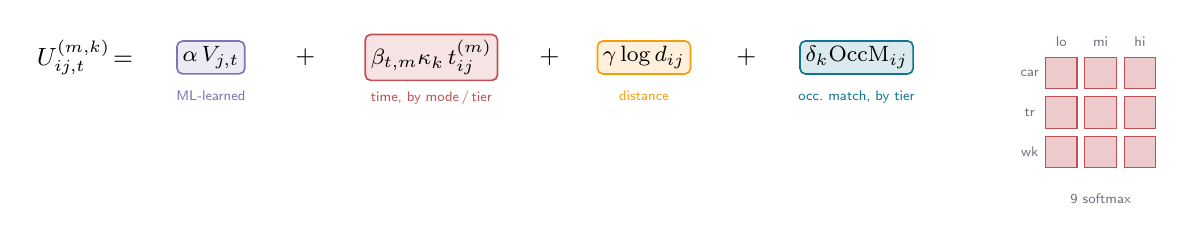
\begin{tikzpicture}[baseline=0]
        \node[font=\sffamily\small] at (-66mm, 0) {$U^{(m,k)}_{ij,t}\!=$};
        \node[draw=cTermV, fill=cTermV!15, rounded corners=2pt, line width=0.6pt,
               inner sep=2pt, font=\sffamily\footnotesize] at (-50mm, 0) {$\alpha\,V_{j,t}$};
        \node[font=\sffamily\small] at (-38mm, 0) {$+$};
        \node[draw=cTermBeta, fill=cTermBeta!15, rounded corners=2pt, line width=0.6pt,
               inner sep=2pt, font=\sffamily\footnotesize] at (-22mm, 0) {$\beta_{t,m}\kappa_k\,t_{ij}^{(m)}$};
        \node[font=\sffamily\small] at (-7mm, 0) {$+$};
        \node[draw=cTermGamma, fill=cTermGamma!15, rounded corners=2pt, line width=0.6pt,
               inner sep=2pt, font=\sffamily\footnotesize] at (5mm, 0) {$\gamma\log d_{ij}$};
        \node[font=\sffamily\small] at (18mm, 0) {$+$};
        \node[draw=cTermDelta, fill=cTermDelta!15, rounded corners=2pt, line width=0.6pt,
               inner sep=2pt, font=\sffamily\footnotesize] at (32mm, 0) {$\delta_k\mathrm{OccM}_{ij}$};
        % term semantics
        \node[font=\sffamily\tiny, text=cTermV, anchor=north] at (-50mm, -3mm) {ML-learned};
        \node[font=\sffamily\tiny, text=cTermBeta, anchor=north] at (-22mm, -3mm) {time, by mode\,/\,tier};
        \node[font=\sffamily\tiny, text=cTermGamma, anchor=north] at (5mm, -3mm) {distance};
        \node[font=\sffamily\tiny, text=cTermDelta, anchor=north] at (32mm, -3mm) {occ.\ match, by tier};
        % mixture grid (right)
        \begin{scope}[shift={(58mm, -2mm)}]
          \foreach \r in {0,1,2}
            \foreach \c in {0,1,2}
              \node[draw=cTermBeta, fill=cTermBeta!30, line width=0.4pt,
                     minimum size=4mm, font=\sffamily\tiny]
                    at (\c*5mm, -\r*5mm) {};
          \foreach \c/\k in {0/lo, 1/mi, 2/hi}
            \node[font=\sffamily\tiny, text=cMuted] at (\c*5mm, 4mm) {\k};
          \foreach \r/\m in {0/car, 1/tr, 2/wk}
            \node[font=\sffamily\tiny, text=cMuted] at (-4mm, -\r*5mm) {\m};
          \node[font=\sffamily\tiny, text=cMuted] at (5mm, -16mm) {9 softmax};
        \end{scope}
      \end{tikzpicture}\\[5pt]
      \scriptsize $P(j|i,t) = \!\!\sum_{m\in\{\mathrm{car,tr,wk}\}}\!\!\!\!\pi_m(i,j)\sum_{k\in\{\mathrm{lo,mi,hi}\}}\!\!\!\!\pi_k(i)\;\mathrm{softmax}_j\,U^{(m,k)}_{ij,t}$
    \end{minipage}};

  % ── ⑤ Cross-entropy loss (absolute X) ──
  \node[modC, anchor=north west] (loss) at (170mm, 0)
    {\begin{minipage}{120mm}
      \centering\textbf{\textcolor{stageCBanner}{\textcircled{\scriptsize 5} Cross-entropy loss + joint backprop}}\\[1pt]
      \scriptsize\textcolor{cIO}{IN: $P(j|i,t),\,F_{ij,t}^{\mathrm{obs}}$}\;\;
      \textcolor{cIO}{OUT: trained $\Theta$}\\[3pt]
      \scriptsize $\mathcal{L} = -\!\!\sum_{i,j,t}\!\! F_{ij,t}\,\log P(j|i,t)$\;\;
      Adam: enc lr 1e-3, head lr 1e-2\\
      \scriptsize $\nabla_\Theta\mathcal{L}$ updates encoder $\Theta_{\text{enc}}$ AND $(\beta,\gamma,\delta,\kappa)$ jointly\\[3pt]
      \includegraphics[width=110mm]{../figures/arch/train_curve_v2.png}\\
      \scriptsize\textit{val CPC = 0.488 (London 2019, 200 ep)}
    \end{minipage}};

  % inner arrows
  \draw[arrInner] (head.east) -- node[arrlbl, above]{$P(j|i,t)$} (loss.west);

\end{scope}

\begin{pgfonlayer}{background}
  \node[rowframe=stageCBg, fit=(row3)] (frameRow3) {};
\end{pgfonlayer}
\node[rowbanner=stageCBanner, anchor=north west]
  at ($(frameRow3.north west)+(8pt, 0pt)$)
  {\textsc{Stage C · Choice head + Loss}\;\,\textmd{\itshape — supervised learning · 77 interpretable parameters}};

% ════════════════════════════════════════════════════════════════════════
%  ROW 4 · TRAINED Θ — output card with 5 sub-cards (full width)
% ════════════════════════════════════════════════════════════════════════

\begin{scope}[local bounding box=row4, shift={(0, -260mm)}]

  % All cards at y=0, with absolute X coords; uniform minimum_height=28mm.
  \node[draw=cParEnc, fill=cParEnc!10, rounded corners=2pt, line width=0.7pt,
         minimum width=52mm, minimum height=28mm,
         font=\sffamily\tiny, text=cParEnc, align=center,
         anchor=north west] (penc) at (0mm, 0)
     {\textbf{$\Theta_{\text{enc}}$}\\\scriptsize\textbf{33{,}026 weights}\\\tiny deep ML, opaque\\\tiny encoder maps $X\!\to\!V_{j,t}$\\\tiny\textit{used by ALL agents in Fig.~2}};
  \node[draw=cParBeta, fill=cParBeta!10, rounded corners=2pt, line width=0.7pt,
         minimum width=58mm, minimum height=28mm,
         font=\sffamily\tiny, text=cParBeta, align=center,
         anchor=north west] (pbeta) at (55mm, 0)
     {\textbf{$\beta_{t,m}$ time sensitivity}\\\scriptsize\textbf{72 params (24h $\times$ 3 modes)}\\\tiny $\beta_{\text{car}}\!=\!{-}.187$\;\;$\beta_{\text{tr}}\!=\!{-}.105$\;\;$\beta_{\text{wk}}\!=\!{-}.049$\\\tiny\textit{agent fetches by mode}};
  \node[draw=cParGamma, fill=cParGamma!10, rounded corners=2pt, line width=0.7pt,
         minimum width=46mm, minimum height=28mm,
         font=\sffamily\tiny, text=cParGamma, align=center,
         anchor=north west] (pgamma) at (116mm, 0)
     {\textbf{$\gamma$ distance decay}\\\scriptsize\textbf{1 param}\\\tiny $\gamma\!=\!{-}.328$\\\tiny universal log-distance penalty\\\tiny\textit{shared by ALL agents}};
  \node[draw=cParDelta, fill=cParDelta!10, rounded corners=2pt, line width=0.7pt,
         minimum width=58mm, minimum height=28mm,
         font=\sffamily\tiny, text=cParDelta, align=center,
         anchor=north west] (pdelta) at (165mm, 0)
     {\textbf{$\delta_k$ occupational matching}\\\scriptsize\textbf{2 free, $\delta_0\!=\!0$ anchor}\\\tiny $\delta_{\text{lo}}\!=\!0$\;\;$\delta_{\text{mi}}\!=\!.20$\;\;$\delta_{\text{hi}}\!=\!.20$\\\tiny\textit{agent fetches by tier}};
  \node[draw=cParKappa, fill=cParKappa!10, rounded corners=2pt, line width=0.7pt,
         minimum width=58mm, minimum height=28mm,
         font=\sffamily\tiny, text=cParKappa, align=center,
         anchor=north west] (pkappa) at (226mm, 0)
     {\textbf{$\kappa_k$ tier scaling on $\beta$}\\\scriptsize\textbf{2 free, $\kappa_0\!=\!1$ anchor}\\\tiny $\kappa_{\text{lo}}\!=\!1.00$\;\;$\kappa_{\text{mi}}\!=\!1.97$\;\;$\kappa_{\text{hi}}\!=\!1.97$\\\tiny\textit{agent fetches by tier}};

\end{scope}

\begin{pgfonlayer}{background}
  \node[rowframe=cParEnc!5, fit=(row4)] (frameRow4) {};
\end{pgfonlayer}
\node[rowbanner=cParEnc, anchor=north west]
  at ($(frameRow4.north west)+(8pt, 0pt)$)
  {\textsc{Trained $\Theta$ — frozen at deployment (bridge to Figure 2)}\;\,\textmd{\itshape Total 33{,}103 params · 77 interpretable (0.23\%)}};

% ════════════════════════════════════════════════════════════════════════
%  MAIN VERTICAL FLOW ARROWS BETWEEN ROWS
% ════════════════════════════════════════════════════════════════════════

\draw[arrFwd] ($(frameRow1.south)+(0, 0)$) --
              node[arrlbl, fill=white, font=\sffamily\small\bfseries]{tensors}
              ($(frameRow2.north)+(0, 0)$);
\draw[arrFwd] ($(frameRow2.south)+(0, 0)$) --
              node[arrlbl, fill=white, font=\sffamily\small\bfseries]{$V_{j,t}$}
              ($(frameRow3.north)+(0, 0)$);
\draw[arrFwd] ($(frameRow3.south)+(0, 0)$) --
              node[arrlbl, fill=white, font=\sffamily\small\bfseries]{trained $\Theta$}
              ($(frameRow4.north)+(0, 0)$);

% ════════════════════════════════════════════════════════════════════════
%  Title and footer
% ════════════════════════════════════════════════════════════════════════

\node[font=\sffamily\bfseries\Large, anchor=south west, text=cText]
  at ($(frameRow1.north west)+(0, 8mm)$)
  {Figure 1 — ML Training Pipeline};
\node[font=\sffamily\itshape\large, anchor=south west, text=cMuted]
  at ($(frameRow1.north west)+(0, 4mm)$)
  {supervised inverse learning of choice parameters from aggregate hourly OD};

\node[font=\sffamily\scriptsize\itshape, text=cMuted, anchor=north west,
       text width=300mm]
  at ($(frameRow4.south west)+(0, -6pt)$)
  {Trained $\Theta$ has \textbf{5 functional categories}:
   $\Theta_{\text{enc}}$ (deep ML, used by anyone going through encoder);
   $\beta_{t,m}$ (time sensitivity, fetched per agent's mode);
   $\gamma$ (distance, shared);
   $\delta_k$ (occ.\ match, fetched per tier);
   $\kappa_k$ (tier scaling on $\beta$, fetched per tier).
   These five types bridge to Figure~2 (ABM forward simulation).};

\end{tikzpicture}

\end{document}
